\section{Break‐Even Penetration Analysis}
\label{sec:Results_BreakEven}

The break-even study identifies the combinations of traffic volume and \ac{mpr} at which \ac{eco-glosa} yields lower mean \ac{co2} emissions than either the \ac{flow-glosa} baseline or the uncontrolled Standard scenario. The numerical results are listed in Tables~\vref{tab:BreakEven_EcoVsFlow} and \vref{tab:BreakEven_EcoVsStd}, while the decision maps are grouped in Figures~\vref{fig:BE_EcoFlow} and \vref{fig:BE_EcoStd}.

\paragraph{\ac{eco-glosa} compared with \ac{flow-glosa}.}
A direct comparison between the two controllers reveals that \ac{flow-glosa} is the superior strategy in the vast majority of scenarios (Table~\vref{tab:BreakEven_EcoVsFlow}). Under the HBEFA4 model, the performance of \ac{eco-glosa} is almost universally negative, indicating higher emissions than \ac{flow-glosa}. It offers only small, sporadic benefits, such as a minor $+1.63~\unit{\gram\per\kilo\metre}$ advantage at $69~\unit{\veh\per\hour}$ and $60\%$ \ac{mpr}, in a landscape otherwise dominated by significant emission penalties. In high-demand scenarios, the outcome is unequivocally negative, with penalties exceeding $-450~\unit{\gram\per\kilo\metre}$, demonstrating that for HBEFA4, there is no reliable operational window for \ac{eco-glosa}.
\mynewline
The PHEMlight5 model provides a clearer, though still limited, window of benefit for \ac{eco-glosa} (Figure~\vref{fig:BE_EcoFlow_PHEM}). The eco-strategy is consistently more beneficial only at very low demands of $69$ to $692~\unit{\veh\per\hour}$. Beyond this, its performance becomes inconsistent and, beginning at a demand of $1385~\unit{\veh\per\hour}$, enters a near-universal deficit. This penalty becomes severe in congestion, reaching as high as $-257~\unit{\gram\per\kilo\metre}$ at $3462~\unit{\veh\per\hour}$. This confirms that even with a more advanced emission model, the throughput-focused logic of \ac{flow-glosa} delivers a better environmental outcome than \ac{eco-glosa} once traffic density increases.

\begin{figure}[htbp]
  \centering
  \begin{subfigure}[b]{0.65\textwidth}
    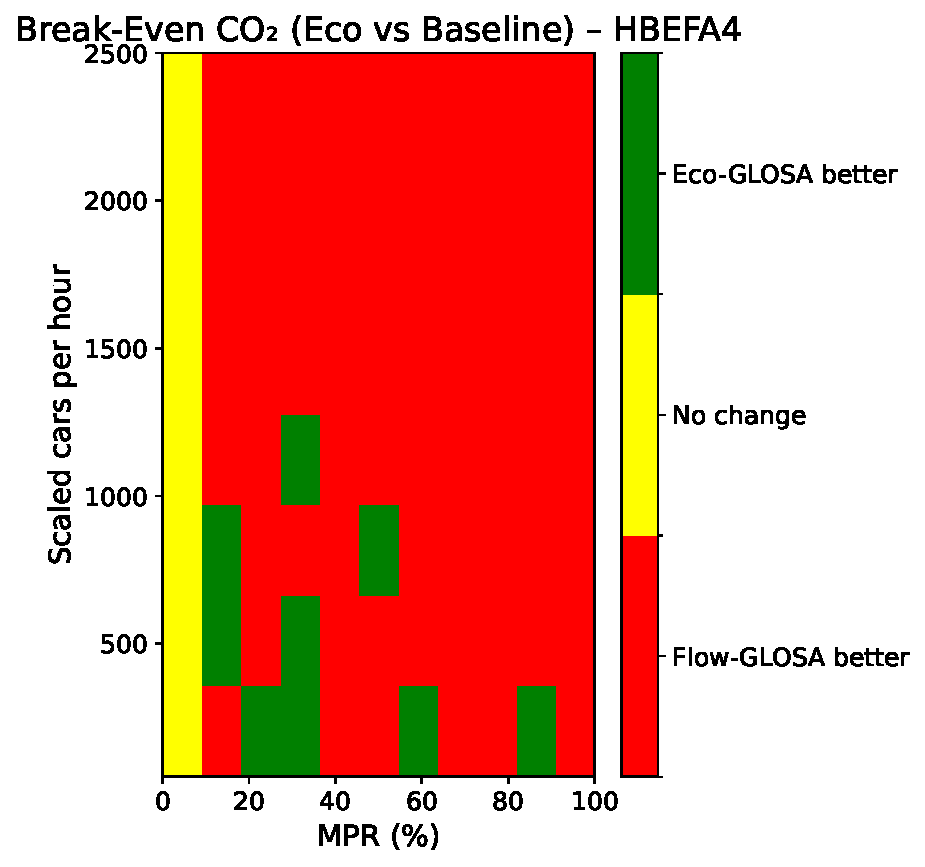
\includegraphics[width=\textwidth]{data/img/BreakEven/BreakEven_CO2_HBEFA4.pdf}
    \caption{Comparison using the HBEFA4 model.}
    \label{fig:BE_EcoFlow_HBEFA4}
  \end{subfigure}
  \begin{subfigure}[b]{0.65\textwidth}
    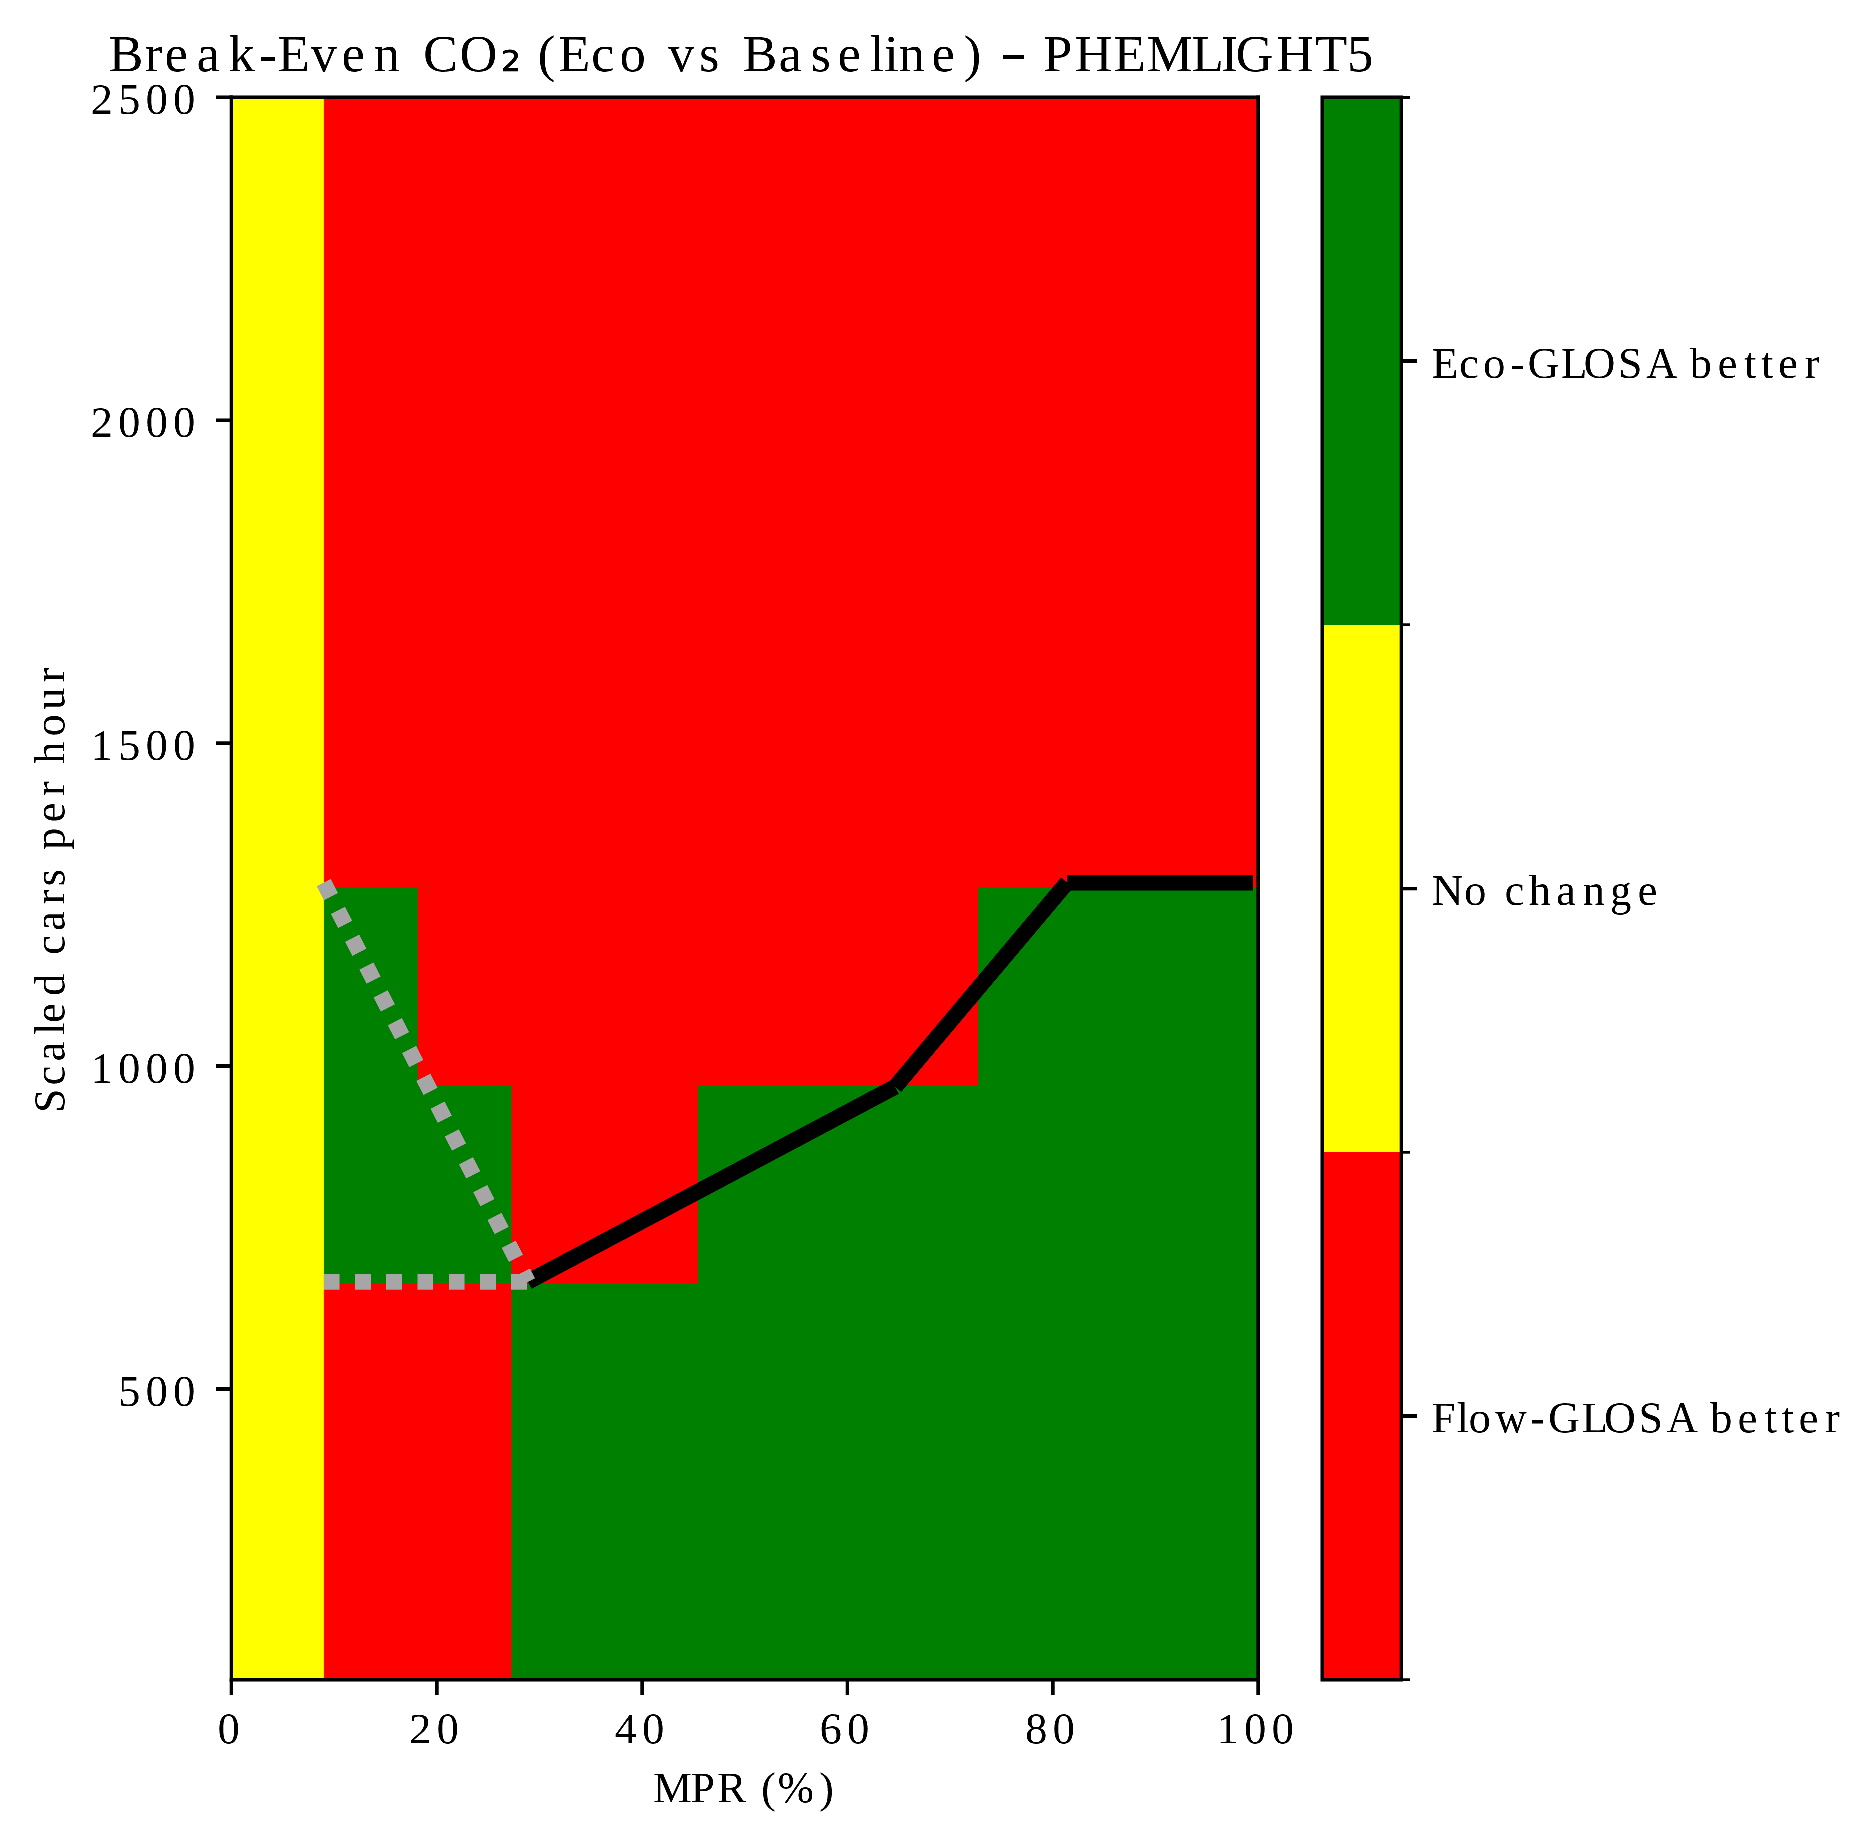
\includegraphics[width=\textwidth]{data/img/BreakEven/BreakEven_CO2_PHEMLIGHT5.pdf}
    \caption{Comparison using the PHEMlight5 model.}
    \label{fig:BE_EcoFlow_PHEM}
  \end{subfigure}
  \caption[Break-even CO2 map: Eco-GLOSA vs. Flow-GLOSA]{Break-even analysis of \ac{co2} emissions, comparing the performance of \ac{eco-glosa} against \ac{flow-glosa}. The heat map visualizes the performance difference across the full parameter space of traffic volume and \ac{mpr}. Green regions denote scenarios where \ac{eco-glosa} is superior (lower emissions), while red indicates that \ac{flow-glosa} is more fuel-efficient.}
  \label{fig:BE_EcoFlow}
\end{figure}

\paragraph{\ac{eco-glosa} compared with Standard.}
When compared to the uncontrolled Standard scenario, \ac{eco-glosa} delivers substantial and consistent emission reductions across all non-congested traffic volumes. Under the HBEFA4 model (Figure~\vref{fig:BE_EcoStd_HBEFA4}), it achieves positive gains across the entire \ac{mpr} spectrum for all demands up to $2077~\unit{\veh\per\hour}$, with a peak reduction of $+10.93~\unit{\gram\per\kilo\metre}$ at $69~\unit{\veh\per\hour}$ and $90\%$ \ac{mpr}. The performance only becomes volatile and negative when entering the high-demand regime at $2769~\unit{\veh\per\hour}$.
\mynewline
Under the PHEMlight5 model, the performance of \ac{eco-glosa} is highly effective in non-congested conditions, creating a broad and consistent region of benefit (Figure~\vref{fig:BE_EcoStd_PHEM}). For all demand levels up to $692~\unit{\veh\per\hour}$, it yields positive outcomes across nearly the entire \ac{mpr} spectrum, with a peak benefit of $+12.03~\unit{\gram\per\kilo\metre}$ recorded at $69~\unit{\veh\per\hour}$. This beneficial performance extends even into the emerging congestion regime. At $1385~\unit{\veh\per\hour}$, while low penetration rates show a minor emission penalty, the controller delivers substantial savings at an \ac{mpr} of $70\%$ and higher, reaching a peak reduction of $+9.17~\unit{\gram\per\kilo\metre}$. A similar pattern is observed at $2077~\unit{\veh\per\hour}$, where the strategy again becomes effective above $70\%$ \ac{mpr}, demonstrating that a high penetration rate can overcome initial instabilities to produce a net environmental benefit. The transition to a universally negative outcome is therefore clearly visible and occurs only upon reaching the high-demand regime of $2769~\unit{\veh\per\hour}$. At this point and into the saturated regime, the controller's inability to manage congestion leads to severe and unavoidable emission penalties that far exceed any of the benefits observed in lighter traffic.

\begin{figure}[htbp]
  \centering
  \begin{subfigure}[b]{0.65\textwidth}
    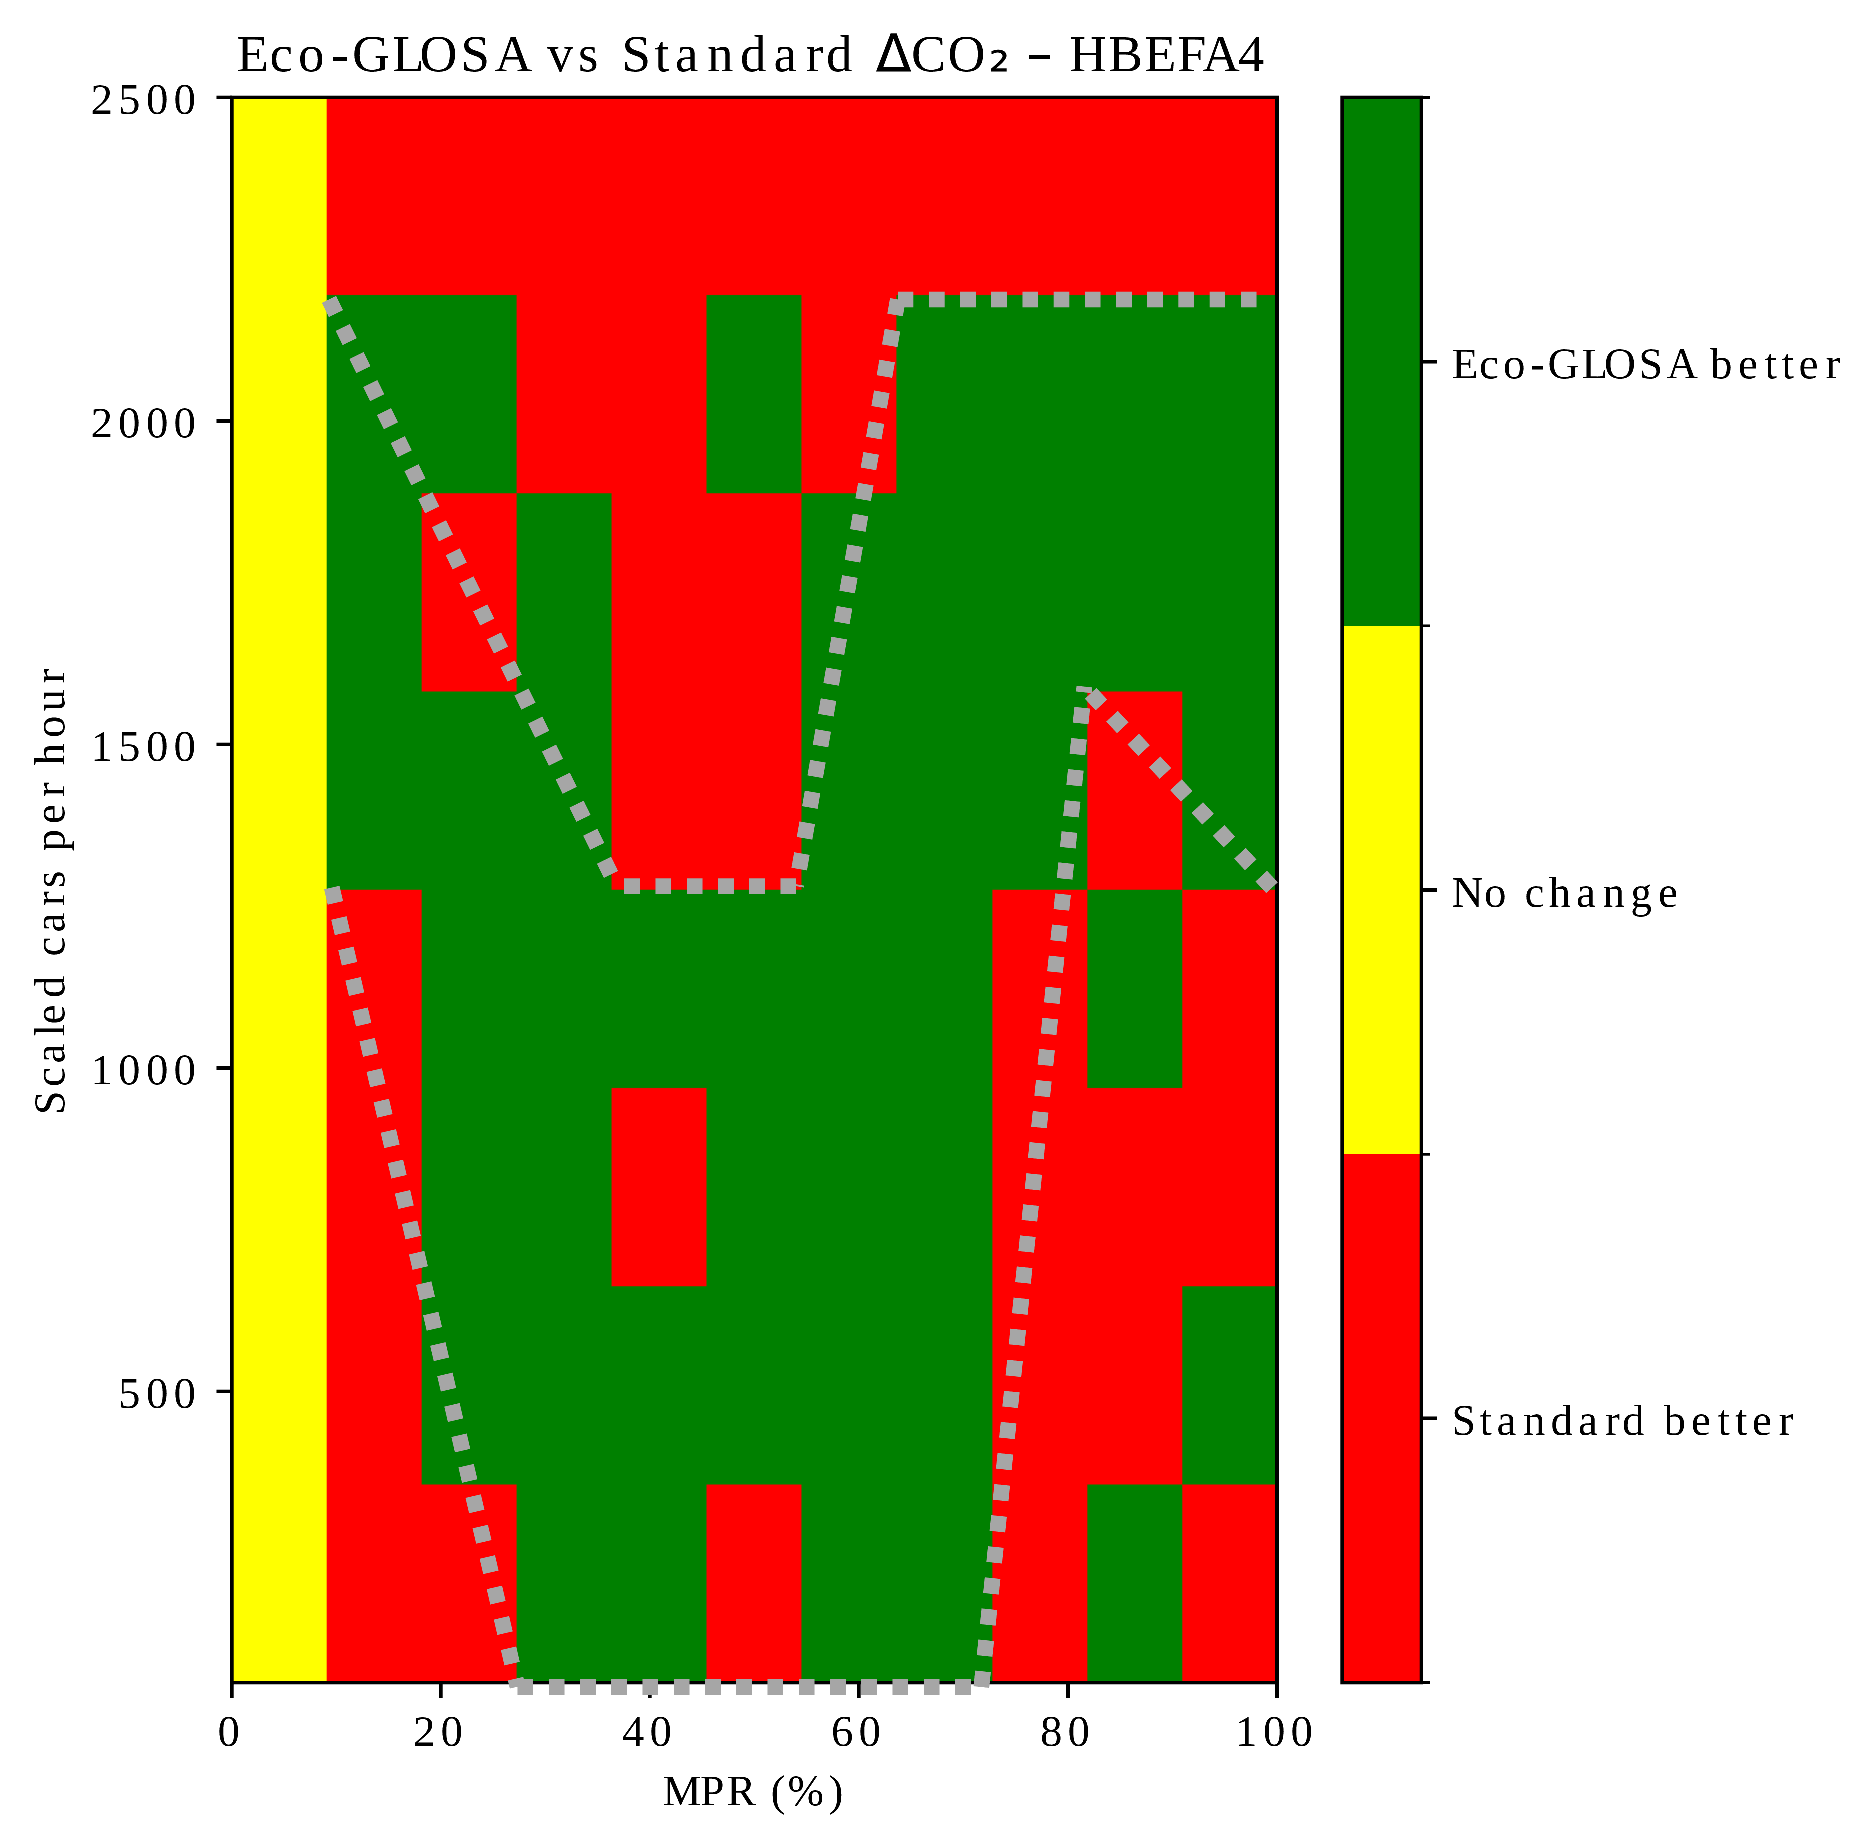
\includegraphics[width=\textwidth]{data/img/BreakEven/delta_CO2_HBEFA4.pdf}
    \caption{Results based on the HBEFA4 model.}
    \label{fig:BE_EcoStd_HBEFA4}
  \end{subfigure}
  \begin{subfigure}[b]{0.65\textwidth}
    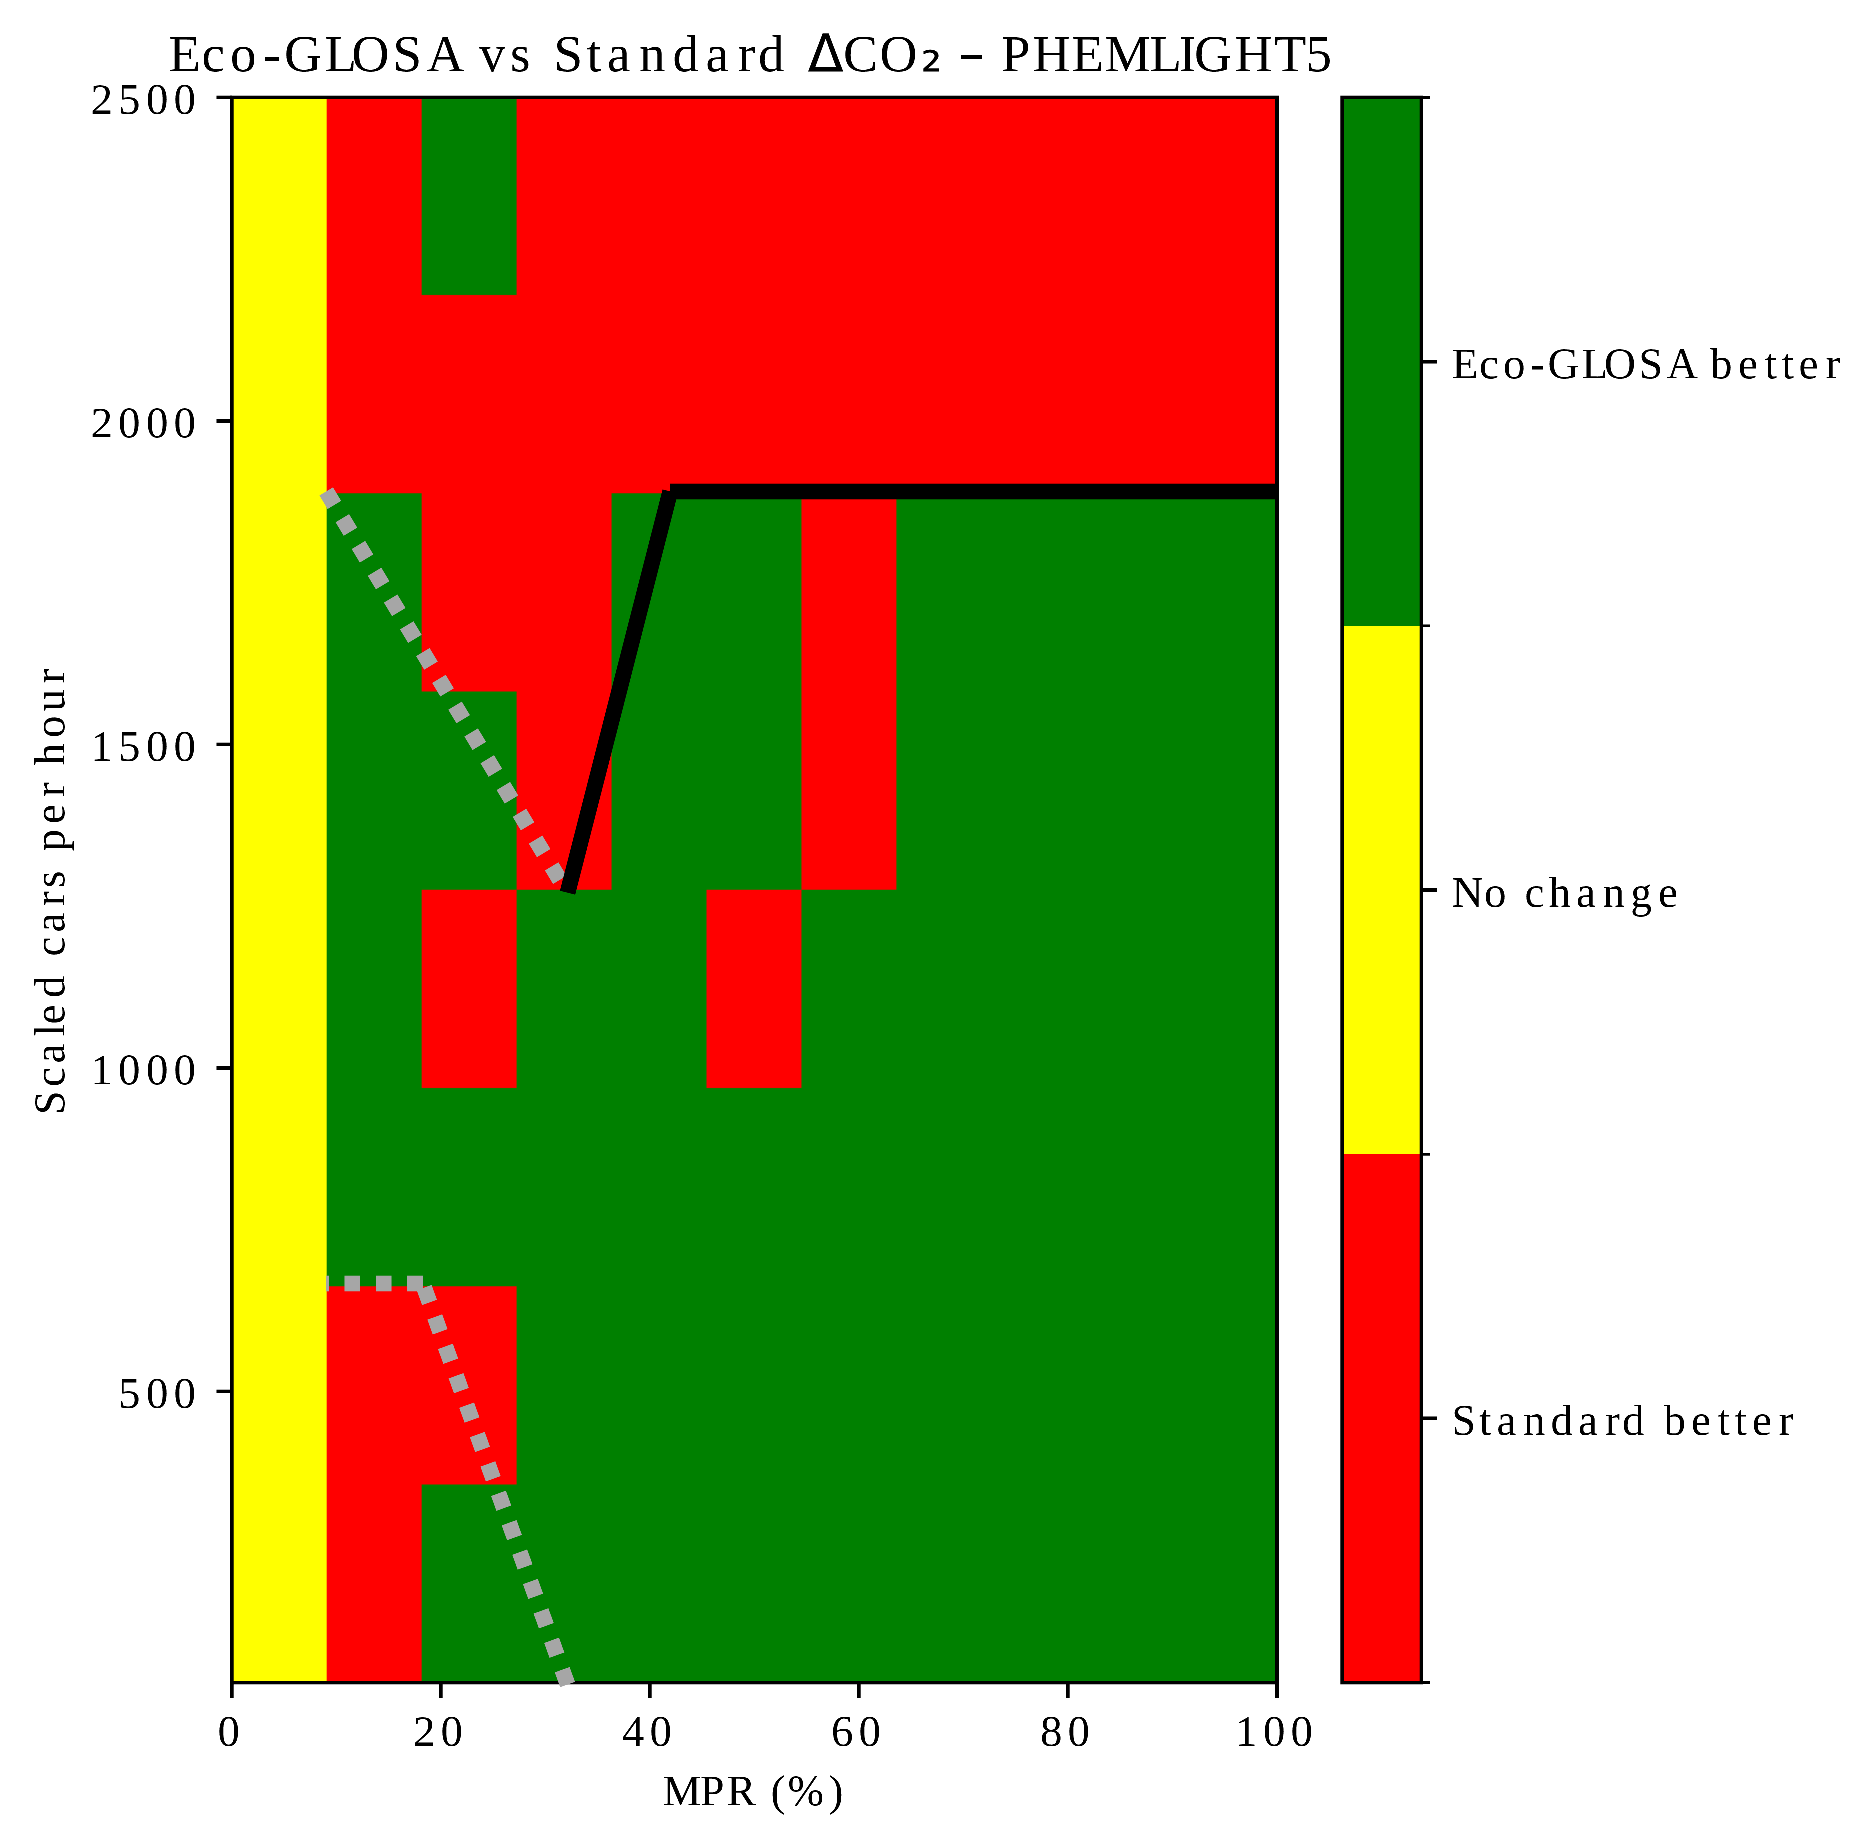
\includegraphics[width=\textwidth]{data/img/BreakEven/delta_CO2_PHEMLIGHT5.pdf}
    \caption{Results based on the PHEMlight5 model.}
    \label{fig:BE_EcoStd_PHEM}
  \end{subfigure}
  \caption[Relative CO2 performance of Eco-GLOSA vs. Standard]{Relative \ac{co2} emission performance of \ac{eco-glosa} compared to the Standard (uncontrolled) scenario. The heat map shows the outcome across all traffic volumes and \ac{mpr} values. Green regions represent a net reduction in emissions for \ac{eco-glosa}, whereas red regions indicate a net increase. The solid black curve traces the path of maximum emission reduction.}
  \label{fig:BE_EcoStd}
\end{figure}

\paragraph{Implications.}
These findings lead to a clear conclusion: while \ac{eco-glosa} is a significant improvement over no \ac{glosa} system at all, the \ac{flow-glosa} strategy is almost always the better choice. The optimal controller strategy is regime-dependent, highlighting a critical trade-off between vehicle-level efficiency and network-level stability. The analysis delineates three distinct operational envelopes.
\mynewline
First, in lightly loaded corridors with demand below approximately $700~\unit{\veh\per\hour}$, both \ac{glosa} strategies are beneficial. In these conditions, there is sufficient spatiotemporal flexibility for vehicles to execute smooth, energy-optimal trajectories without negatively impacting each other. When evaluated with the more physically accurate PHEMlight5 model, the \ac{eco-glosa} controller is the preferable strategy in this regime. It consistently outperforms \ac{flow-glosa} at demands up to $346~\unit{\veh\per\hour}$, delivering a more significant emission reduction. This advantage diminishes as demand increases, with \ac{flow-glosa} becoming the more stable choice as the corridor approaches the $700~\unit{\veh\per\hour}$ threshold.
\mynewline
Second, the transition range ($700$--$2077~\unit{\veh\per\hour}$) represents a highly sensitive, \enquote{knife-edge} condition. Here, the ineffective optimisation of \ac{eco-glosa} can create voids in the traffic stream, triggering stop-and-go waves that increase emissions. The risk is highest at low-to-moderate penetration rates, where equipped vehicles conflict with the uncoordinated flow of standard vehicles. As the results show, the emission penalties in this regime can be an order of magnitude greater than the best-case savings in light traffic. Therefore, the \ac{flow-glosa} controller is the more robust and reliable choice, as it consistently outperforms \ac{eco-glosa} and prevents these instabilities.
\mynewline
Finally, in saturated corridors with demand above $2700~\unit{\veh\per\hour}$, the primary objective shifts from efficiency to preventing network collapse. In this regime, the \ac{flow-glosa} strategy is clearly preferred. Its ability to suppress stop-and-go waves by maximising throughput is the most effective approach for achieving system-wide environmental benefits. By preventing the severe stop-start cycles that dominate emissions in a jam, it delivers profound emission reductions of over $66\%$. This underscores that a static, \enquote{one-size-fits-all} \ac{glosa} controller is suboptimal. A practical and readily implementable advancement would be a hybrid, adaptive system that leverages real-time traffic state data to dynamically switch its core objective --- prioritising energy efficiency in light traffic only when it does not compromise the robust, throughput-maximising logic required as congestion builds.

\paragraph{Key Takeaways.}
\begin{enumerate}
    \item \textbf{\ac{flow-glosa}: The Robust Choice:} A direct comparison shows that the throughput-oriented \ac{flow-glosa} yields lower \ac{co2} emissions than \ac{eco-glosa} in the vast majority of scenarios. The operational window where \ac{eco-glosa} is preferable is narrow and limited to light traffic under specific conditions.
    \item \textbf{Benefit of \ac{eco-glosa} over Standard:} Compared to an uncontrolled intersection, \ac{eco-glosa} provides consistent and significant emission reductions, but only in reliably unsaturated traffic conditions ($< 2700~\unit{\veh\per\hour}$).
    \item \textbf{High-Demand Liability:} The primary finding is that \ac{eco-glosa}'s design becomes a critical liability in high-demand traffic. Its failure to prioritise throughput induces congestion, which completely negates and vastly outweighs any potential fuel-saving benefits.
    \item \textbf{Deployment Strategy is Regime-Dependent:} The analysis defines clear operational envelopes. While \ac{eco-glosa} is viable in light traffic, its risk of inducing congestion makes \ac{flow-glosa} the necessary choice for corridors operating near or at capacity to ensure network stability and achieve the best environmental outcome.
    \item \textbf{Adaptive Systems as a Practical Advancement:} The findings suggest that a practical and readily implementable advancement is a hybrid, adaptive system that can prioritise eco-driving principles in low-density traffic and transition to a throughput-maximising strategy as congestion builds.
\end{enumerate}

\begin{table}[htb]
  \centering
  \caption[CO2 Emission Difference: Eco-GLOSA vs. Flow-GLOSA]{Difference in CO\textsubscript{2} emissions, measured in $\unit{\gram\per\kilo\metre}$, between the \ac{eco-glosa} and \ac{flow-glosa} controllers. The values are tabulated across all simulated traffic volumes and market penetration rates. A positive value signifies that \ac{eco-glosa} achieved a better fuel economy.}
  \label{tab:BreakEven_EcoVsFlow}
  \resizebox{\textwidth}{!}{%
    \begin{tabular}{r l *{12}{r}}
      \toprule
      Vehicles & Fuel        & \textbf{0\% (Standard)} & 10\%    & 20\%    & 30\%      & 40\%      & 50\%      & 60\%        & 70\%    & 80\%      & 90\%      & 100\%     \\
      \midrule
      69   & HBEFA4      & \textbf{149.99}       & -0.96   & \textbf{0.19}    & \textbf{0.68}      & -1.43     & -1.02     & \textbf{1.63}        & -0.61   & -1.21     & \textbf{1.41}      & -2.92     \\
      138  & HBEFA4      & \textbf{148.70}       & \textbf{0.04}    & -0.15   & \textbf{1.40}      & -1.12     & -0.28     & -0.13       & -0.71   & -0.82     & -0.10     & -0.06     \\
      346  & HBEFA4      & \textbf{147.86}       & \textbf{0.43}    & -0.57   & -1.48     & -0.32     & \textbf{0.28}      & -0.22       & -1.16   & -1.77     & -1.32     & -1.69     \\
      692  & HBEFA4      & \textbf{148.06}       & -1.19   & -0.18   & \textbf{0.10}      & -0.74     & -0.42     & -0.85       & -1.26   & -2.06     & -1.72     & -1.67     \\
      1385 & HBEFA4      & \textbf{149.86}       & -0.57   & -0.51   & -0.71     & -0.80     & -1.28     & -2.18       & -2.01   & -2.68     & -1.16     & -2.89     \\
      2077 & HBEFA4      & \textbf{152.91}       & -0.89   & -1.30   & -2.38     & -2.03     & -2.60     & -3.62       & -2.82   & -2.94     & -3.33     & -3.51     \\
      2769 & HBEFA4      & \textbf{158.44}       & -4.18   & -2.97   & -118.09   & -73.85    & -3.38     & -272.42     & -4.30   & -3.72     & -3.76     & -4.52     \\
      3462 & HBEFA4      & \textbf{426.68}       & -61.24  & -84.09  & -102.44   & -129.10   & -156.27   & -351.31     & -206.47 & -450.77   & -449.50   & -460.41   \\
      \midrule
      69   & PHEMlight5 & \textbf{155.51}       & -1.13   & \textbf{2.35}    & \textbf{2.14}      & \textbf{2.19}      & \textbf{1.72}      & \textbf{1.26}        & \textbf{3.35}    & \textbf{1.94}      & \textbf{3.54}      & \textbf{2.88}      \\
      138  & PHEMlight5 & \textbf{155.28}       & -0.40   & \textbf{0.66}    & \textbf{3.63}      & \textbf{2.34}      & \textbf{4.10}      & \textbf{1.87}        & \textbf{0.51}    & \textbf{2.89}      & \textbf{5.48}      & \textbf{5.47}      \\
      346  & PHEMlight5 & \textbf{156.60}       & \textbf{0.84}    & -1.28   & -0.15     & \textbf{0.80}      & \textbf{1.92}      & \textbf{0.39}        & \textbf{1.46}    & \textbf{1.13}      & \textbf{3.06}      & \textbf{1.41}      \\
      692  & PHEMlight5 & \textbf{157.36}       & -0.59   & -1.25   & -1.02     & -0.16     & -0.65     & -0.60       & -0.06   & -0.39     & \textbf{1.06}      & \textbf{2.85}      \\
      1385 & PHEMlight5 & \textbf{159.38}       & -2.13   & -3.52   & -4.83     & -4.03     & -4.56     & -6.19       & -3.65   & -2.94     & \textbf{0.28}      & \textbf{0.20}      \\
      2077 & PHEMlight5 & \textbf{162.83}       & -3.92   & -3.87   & -5.57     & -6.67     & -5.45     & -7.11       & -7.15   & -4.23     & -3.61     & -2.51     \\
      2769 & PHEMlight5 & \textbf{168.29}       & -34.25  & -85.80  & -138.25   & -159.30   & -179.71   & -172.00     & -189.98 & -173.30   & -198.99   & -124.50   \\
      3462 & PHEMlight5 & \textbf{344.88}       & -40.55  & -55.85  & -63.07    & -74.91    & -88.61    & -197.81     & -112.43 & -249.66   & -255.74   & -257.28   \\
      \bottomrule
    \end{tabular}%
  }
\end{table}

\begin{table}[htb]
  \centering
  \caption[CO2 Emission Difference: Eco-GLOSA vs. Standard]{Difference in CO\textsubscript{2} emissions, measured in $\unit{\gram\per\kilo\metre}$, between the \ac{eco-glosa} controller and the uncontrolled Standard scenario. The values are tabulated across all simulated traffic volumes and market penetration rates. A positive value indicates an emission reduction achieved by \ac{eco-glosa}.}
  \label{tab:BreakEven_EcoVsStd}
  \resizebox{\textwidth}{!}{%
    \begin{tabular}{r l *{12}{r}}
      \toprule
      Cars & Fuel        & \textbf{0\% (Standard)} & 10\%    & 20\%    & 30\%      & 40\%      & 50\%      & 60\%      & 70\%      & 80\%      & 90\%      & 100\%     \\
      \midrule
      69   & HBEFA4      & \textbf{149.99}       & \textbf{4.83}  & \textbf{2.46}  & \textbf{5.40}  & \textbf{5.70}  & \textbf{3.18}  & \textbf{6.54}  & \textbf{8.50}  & \textbf{6.13}  & \textbf{10.93} & \textbf{7.52}  \\
      138  & HBEFA4      & \textbf{148.70}       & \textbf{3.15}  & \textbf{2.70}  & \textbf{4.56}  & \textbf{5.37}  & \textbf{5.47}  & \textbf{6.74}  & \textbf{8.11}  & \textbf{6.34}  & \textbf{7.62}  & \textbf{8.36}  \\
      346  & HBEFA4      & \textbf{147.86}       & \textbf{0.60}  & \textbf{0.60}  & \textbf{0.38}  & \textbf{2.63}  & \textbf{3.13}  & \textbf{4.94}  & \textbf{3.72}  & \textbf{5.19}  & \textbf{6.08}  & \textbf{7.15}  \\
      692  & HBEFA4      & \textbf{148.06}       & \textbf{0.08}  & \textbf{2.06}  & \textbf{2.27}  & \textbf{2.88}  & \textbf{3.71}  & \textbf{5.07}  & \textbf{5.04}  & \textbf{5.99}  & \textbf{6.90}  & \textbf{6.89}  \\
      1385 & HBEFA4      & \textbf{149.86}       & \textbf{0.16}  & \textbf{0.64}  & \textbf{1.87}  & \textbf{3.15}  & \textbf{3.82}  & \textbf{4.40}  & \textbf{5.52}  & \textbf{6.49}  & \textbf{7.79}  & \textbf{8.00}  \\
      2077 & HBEFA4      & \textbf{152.91}       & \textbf{1.00}  & \textbf{0.71}  & \textbf{1.85}  & \textbf{3.36}  & \textbf{4.34}  & \textbf{5.54}  & \textbf{7.28}  & \textbf{8.30}  & \textbf{9.69}  & \textbf{9.44}  \\
      2769 & HBEFA4      & \textbf{158.44}       & -2.17 & \textbf{0.03}  & -112.49 & -65.81 & \textbf{7.61}  & -260.65 & \textbf{9.24}  & \textbf{10.26} & \textbf{12.29} & \textbf{12.54} \\
      3462 & HBEFA4      & \textbf{426.68}       & -51.04 & -69.38 & -94.30  & -107.10 & -120.80 & -148.47 & -140.95 & -170.35 & -166.61 & -176.51 \\
      \midrule
      69   & PHEMlight5 & \textbf{155.51}       & \textbf{3.56}  & \textbf{3.14}  & \textbf{7.14}  & \textbf{8.82}  & \textbf{5.46}  & \textbf{6.34}  & \textbf{10.97} & \textbf{7.50}  & \textbf{12.03} & \textbf{10.31} \\
      138  & PHEMlight5 & \textbf{155.28}       & \textbf{2.50}  & \textbf{2.22}  & \textbf{5.37}  & \textbf{6.62}  & \textbf{7.83}  & \textbf{6.47}  & \textbf{7.53}  & \textbf{7.47}  & \textbf{10.10} & \textbf{11.18} \\
      346  & PHEMlight5 & \textbf{156.60}       & \textbf{0.75}  & -0.55 & \textbf{0.79}  & \textbf{2.87}  & \textbf{3.60}  & \textbf{4.65}  & \textbf{5.37}  & \textbf{7.32}  & \textbf{9.03}  & \textbf{9.21}  \\
      692  & PHEMlight5 & \textbf{157.36}       & \textbf{0.21}  & \textbf{0.30}  & \textbf{0.16}  & \textbf{1.73}  & \textbf{1.95}  & \textbf{3.85}  & \textbf{4.51}  & \textbf{6.10}  & \textbf{8.12}  & \textbf{9.42}  \\
      1385 & PHEMlight5 & \textbf{159.38}       & -2.23 & -3.33 & -3.61 & -1.66 & -1.19 & -1.32 & \textbf{1.80}  & \textbf{4.38}  & \textbf{7.30}  & \textbf{9.17}  \\
      2077 & PHEMlight5 & \textbf{162.83}       & -2.94 & -3.36 & -3.25 & -3.52 & -0.74 & -0.05 & \textbf{0.80}  & \textbf{4.88}  & \textbf{7.24}  & \textbf{8.20}  \\
      2769 & PHEMlight5 & \textbf{168.29}       & -32.96 & -84.59 & -135.11 & -154.40 & -171.80 & -163.38 & -179.44 & -162.27 & -185.64 & -109.83 \\
      3462 & PHEMlight5 & \textbf{344.88}       & -32.96 & -43.13 & -54.31 & -57.55 & -63.32 & -63.75 & -65.57 & -64.29 & -67.16 & -67.90 \\
      \bottomrule
    \end{tabular}%
  }
\end{table}
